\documentclass[12pt]{article}
\usepackage{a4wide}
\usepackage{NotationStyle}
\usepackage[]{algorithm2e}
%\usepackage[noend]{algorithmic}
\usepackage[english]{babel}
\usepackage{amsmath,amssymb,mathrsfs,mathtext}
\usepackage{graphics,graphicx,epsfig}
\usepackage{epstopdf}
\usepackage{fancybox,fancyhdr}
\usepackage{enumerate}
\usepackage{array}
\usepackage{color, soul}
\usepackage{longtable}
\usepackage[normalem]{ulem}

\newcommand{\argmax}{\mathop{\rm arg\,max}\limits}

\renewcommand{\baselinestretch}{1.3}
\begin{document}
\title{Feature generation for multiscale time series forecasting multimodels}
\author{LIG}%Radoslav Neychev, Eric Gaussier and Vadim Strijov}
\date{Technical report (pre-draft)}
\maketitle

\section*{Notation}
\begin{longtable}{p{4cm}p{12cm}}
$\fD=\{\bs, \bs', \bs'', \dots\}$ & large set of time series \\
$\bar{\bs}$ & special case of time series $\bs$ for classification \\
$T_{\max}$ & maximum number of time stamps \\
$\dtp$ & local prehistory \\
$\dtr$ & defines time period (requested) for prediction \\
$\bs_i = [\y_i|\x_i]$ & local ($t_i$) segment of the time series $\bs$ \\
$\bX^{*}$, $\bx_i^{*} = [\y_i, \y'_i, \dots |\x_i, \x'_i, \dots]$ & object-feature matrix \\
$\bY$, $\bX$ & target matrix, feature matrix \\
$m$ & number of objects $\bx_i^{*}$ extracted from $\fD$ \\
$r$ & dimensionality of the target vector $[\y_i, \y'_i, \dots]$ \\
$n$ & dimensionality of the feature vector $[\x_i, \x'_i, \dots]$ \\
$\bx_0^{*} = [\hat{y}|\bx_0]$ & a testing object? \\
$\cJ = {1,\dots, n}$ & feature index set \\
$\cA \subset \cJ$ & the subset of feature indices \\ 
$\fx_k(\w_{\cA_k}, \x)$, $k=1,\dots,K$ & regression model, defined for a subset $\cA_k$ \\
$\w_{\cA_k}$ & model parameters (alternatively, $\w_k$)\\
$\boldsymbol{\pi} = [\pi_{i1}, \dots, \pi_{iK}]$ & vector of correspondence \\
$\cI = \{1, \dots, m\} = \cB_0 \sqcup_k \cB_k$ & set of object indices \\
$\cB_0$ & test set \\
$\cB_k$, $k=1,\dots,K$ & training sets \\
$Q$ & quality function \\
$S$ & error function \\ 
$g=g(\bb,s)$ parametric functions for feature transformation \\
$\mathfrak{G} = \{g:\bs\to\vf\}$ & set of feature transformations \\
$\vf=[\vf^\prime,\vf^{\prime\prime},\dots]$ & generated feature vector \\ 
$\veps = \by - \hat{\by}$ & vector of residuals \\
$\bc^\prime_1,\dots,\bc^\prime_P$ & $k$-means centroids \\
$\mathbf{H}^{*}$ & Hankel matrix \\
$\bth = [\w_1, \dots, \w_k, \boldsymbol{\pi}, \beta]$ & parameters of the mixture model \\
$z_{ik}$, $\gamma_{ik}$ & latent (correspondence) variables and their expectations (mixture models) \\
\end{longtable}

\section{Introduction}
The paper investigated behavior of a device, a member of the internet of things. A device is monitored by a set of sensors, which produces large amount of multiscale time series during its lifespan. These time series have various time scales, due to measurements could perform over each millisecond, day, week, etc.  The main goal is to forecast the next state of a device.

The investigation assumes the following conditions for a single device unit time series: there are large set of multiscale time series; the sampling rate of a time series is fixed; each time series has its own forecast horizon. Examples of this kind of time series are listed below. \hl{(list)}

To make an adequate forecasting model hold the following hypothesis: the time history is sufficient long; the time series have auto- and cross-correlation dependencies. The model is static, so there exists a history of optimal size. Each time series could be interpolated by some local model (constant, piece-wise), a that there exist a local approximation model, which could be applied in the case of local data absence.

To forecast time series under the listed conditions autoregressive models constructed in next TODO (list and review state of the art).

\section{Problem statement}
\hl{There give a large set of time series~$\fD=\{\bs\}$, where each real-valued time series~$\bs$  has its own sample rate. Assuming each time series could be interpolated introduce a joint sample rate and assign each series~$\bs$ has minimum one and maximum~$T_{\max}$ samples for one time-tick of this rate.} Introduce joint time-scale and split it to the following parts, as Fig.~\label{TimeScale} shows. The first part is the history itself, the second part is the local history, which forms an object of the �object-feature� matrix to make a forecast. The third part is a requested forecast time-segment~$\Delta t_\text{r}$ and the last one is a forecast horizon.

%\begin{define}
Forecast horizon is a time segment~$\Delta t_\text{h}$, which brings an adequate (TODO explain it) forecast~$\bs(\Delta t_\text{h})$ in comparison to the real historical values~$\hat{\bs}(\Delta t_\text{h})$.
%\end{define}

Assign to the requested forecast time-segment~$\Delta t_\text{r}$ a new vector~$\by$ of forecasts. This vector contains forecasts to all time series of the set~$\{\bs\}$. The value of~$\Delta t_\text{r}$ is given so that each time series~$\bs$ has minimum one sample. A~proportion of~$T_{\max}$ samples for time series of high frequency sample rates could be considered, too.

Form an object set at a set of the vectors~$\{\bx\}$, where each vector~$\{\bx\}$ collects all the time series over the time~$\Delta t_\text{p}$. Here~$\text{p}$ stands for the local \emph{prehistory}. The vector could (with no necessity) include samples from previous history of any time series as well as any derivatives, which are called generated features. Construct the ``object-feature'' matrix~$\bX^*$ for the multiscale autoregressive problem statement as follows. Denote~$i$-th element from the sample set as a row-vector
\[
\bs_i^\prime = [\by_i^\prime, \bx_i^\prime] = [\underbrace{s(t_i),\dots,s(t_i-\Delta t_\text{r})),}_{\by_i^\prime}
\underbrace{\dots,s(t_i-\Delta t_\text{r}-\Delta t_\text{p})}_{\bx_i^\prime}],
\]
where~$s(t)$ is an element of time series~$\bs$. Denote the other time series from~$\fD$ in this segment~$(t_i,\dots,t_i-\Delta t_\text{r}-\Delta t_\text{p})$ as~$\by_i^{\prime\prime}, \bx_i^{\prime\prime},\dots$%,\by_i^{\prime\prime\prime},\bx_i^{\prime\prime\prime}$
and form the matrix
 \[
\bX^*=\left[
\begin{array}{lll|lll}
\hat{\by^\prime} & \hat{\by}^{\prime\prime} & \dots & \bx_0^\prime & \bx_0^{\prime\prime} & \dots \\
\hline
\by_1^\prime & \by_1^{\prime\prime} & \dots & \bx_1^\prime & \bx_1^{\prime\prime} & \dots \\
\vdots & \vdots & \ddots & \vdots & \vdots & \ddots \\
\by_m^\prime & \by_m^{\prime\prime} & \dots & \bx_m^\prime & \bx_m^{\prime\prime} & \dots \\
\end{array}
\right]
=\left[
\begin{array}{c|c}
 \underset{1{\times}r}{\hat{\by}} & \underset{1{\times}n}{\x_0} \\
 \hline
 \underset{m{\times}r}\bY & \underset{m{\times}n}\bX \\
\end{array}
\right].
\]
Denote a row from the pair~$\bY,\bX$ as $\by,\bx$ and call these vectors the target and the features. As one must forecast all elements from the target~$\by$, only a few elements from the features~$\bx$ are supposed to be informative in terms of the forecast quality. Denote the index set~$\cJ=\{1,\dots,n\}$ and select the subset of the indexes~$\cA\in\cJ$.
Introduce the forecasting model
\[
\hat{\by}_i = \sum_{k=1}^K \pi_{ik} \mathbf{f}_k  (\bw_{\mathcal{A}_k}, \bx_{i\mathcal{A}_k})
\]
as some linear combination of~$K$ models and call it the \emph{multimodel}. Each model~$\fx_k$ has its parameters~$\bw_k$ and selected features~$\bx_{\cA_k}$. The coefficient~$\pi_{ik}$ set a vector~$ \bx_i$ in correspondence to the  model~$\fx_k$, so that
\[
\sum_{k=1}^K \pi_{ik}  = 1 \quad\text{for}\quad i\in\cI = \{1,\dots,m\}
\]
with two options are to be considered:~$\pi\in\{0,1\}$ and~$\pi\in[0,1]$.
Let the forecasting error be
\[
S=\sum_{i\in\cB_0} \|\hat{\by}_i - \by_i\|_1,
\]
where the set of object indexes~$\cI$ is splatted to the test set~$\cB_0$ and the train sets,
\[
\cI = \cB_0\mathop{\sqcup}\limits_{k=1}^K \cB_k.
\]

State the forecasting problem as a problem to minimize the error function~$S$ given models~$\fx_1,\dots,\fx_K$ by optimizing matrix $\Pi = [\pi_{ik}]$, finite sets~$\cA_1,\dots,\cA_K$ and model parameters~\hl{$\bw_1,\dots,\bw_K$} on the sample set with indexes~$\cI\setminus\cB_0$.

\section{Special case of the problem}
A special case of the problem is an early warning forecasting. There is a special time series~$\bar{\bs}$ with its elements~$\bar{s}\in\{0,1\}$. Here zero is interpreted as a \emph{normal state} of the system and one meas the system goes from normal to the \emph{abnormal} state without return over time~$t$.
The problem is to maximize the lapse of the time segment
\[ \| \Delta t_\text{r} \| \to\max,\]
where the vector
\[
[\bar{\bs}(\Delta t_\text{h}), \bar{\bs}(\Delta t_\text{r})] = [0,\dots,0,0,\dots,0,1],
\]
which means the system was in the normal state before it changes. Since the quality~$Q$ of forecasting time series~$\bar{\bs}$ depends on~$\| \Delta t_\text{r} \|$ (the letter time lapse before the warning the higher the forecasting quality~[ref]) the minimum level of quality must be set. Let the minimum forecasting quality be
\[
Q \left\{
\bigl(\hat{\bs}_i(\Delta t_\text{r}),\bar{\bs}_i(\Delta t_\text{r})\bigr)
\;|\;
i\in\cB_0
\right\} = \text{AUC} = Q_\text{req}.
\]

\section{Time searies resampling}
For the time series of sample rate that is changing, unstable, non-rational to the common rate as well as for the time series with missing values the following procedure should be applied.

Let the time~$t$ be in continuous set~$\mathbb{R}_+^1$ and the time series~$s$ be piece-wise constant. There are three possibilities to create such time series from a discrete-values one: 1) the constant goes after the sample~$s(t)$, 2) before the sample, 3) in the neighborhood of the sample. See red, green and blue lines in the Figure~\ref{fig_resample1}.

\begin{figure}[!hp]
\centering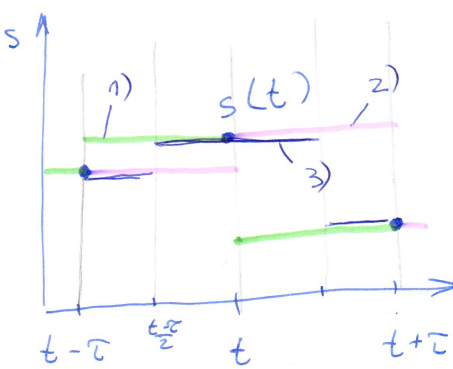
\includegraphics[width=0.5\textwidth]{resample1.png}
\label{fig_resample1}
\caption{Piece-wise representation of a time series}
\end{figure}

This assumptions helps introducing a new sampling rate and eliminates the problem of missing values, since the previous (next, current in the terms of Fig.~\ref{fig_resample1}) value holds continuously until the following comes. The constant model could be developed into more comples one: a piece-wise, quadratic or cubic spline with its nodes in the time-ticks or over the time-ticks according to the following criterions: 1) Nyquist�Shannon theorem, 2) Fisher-Neyman theorem. The following optimization problem returns the new sampling rate:
\[
\text{todo}
\]
This fixed rate is used to obtain a resampled time series with regular time-ticks.

\begin{figure}[!t]
\centering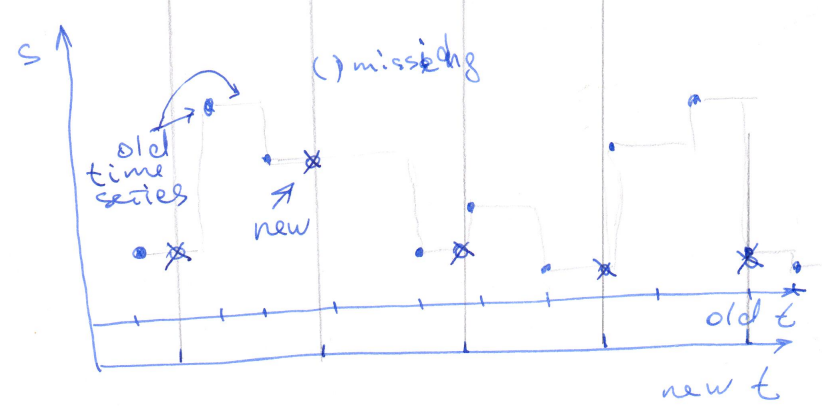
\includegraphics[width=0.9\textwidth]{resample2.png}
\label{fig_resample2}
\caption{Resample time series of variating sample rate into the fixed one with the optimal period}
\end{figure}

\subsection{Nyquist�Shannon  resampling criterion}
TODO

\subsection{ Fisher-Neyman resampling criterion}
TODO
\subsection{Wavelet resampling}
In signal processing a common way to change resolution of a signal is to use a combination of upsampling and decimation (FFT \hl{wavelet transform} and downsampling). Suppose that desired sampling rate $u$ is fixed, that is, we would like to approximate $U = uT_{\max}$ uniformly sampled observations $\tilde{s}(\tilde{t}_i), \; i = 1, \dots U$ of the time series $s(t_i), \; i=1, \dots, T_{\max}$. Let $G = \{t_1, \dots, T_{\max}\}$ and $\tilde{G} = \{\tilde{t}_1, \dots, T_{\max}\}$ denote the current and the desired grids.
The first step to rescaling $\bs \rightarrow \tilde{s}$ is the piecewise approximation $\hat{\bs}$ (see Fig.~\ref{fig_resample1} and Fig.~\ref{fig_resample2}) of $\bs$ at $\hat{G} = G \cup \tilde{G}$. To increase the smoothness of piecewise approximation $\hat{\bs}$ we apply low pass FFT \hl{wavelet} filtering to $\hat{\bs}$ and then downsample the output to $\tilde{G}$.

\begin{algorithm}[ht]
\textbf{TimeSeriesRescaling()}

 \KwData{$\bs$. Parameters: desired grid $\tilde{G} = \{\tilde{t}_1, \dots \tilde{t}_U\}$.}
 \KwResult{Resamples time series $\tilde{\bs}$.}
 Form the new grid $\hat{G} = G \cup \tilde{G}$\;
 Upsample time series, using piecewise approximation:
 
 $\quad \hat{\bs} \leftarrow \text{~\textbf{Piecewise}}(\bs, G, \tilde{G})$\;
 Zero-pad $\hat{\bs}$, so that $|\hat{G}| = 2^{N}$, where $N = \lceil \log_2(|\hat{G}|)\rceil$\;
 Apply low pass filtering $\hat{\bs}$:
 
 $\quad \hat{\bs}_{\text{lf}} = \text{\textbf{LowPassFFTFiltering}}(\hat{\bs})$ \;
 Downsample $\hat{\bs}_{\text{lf}}$ to $\tilde{G}$:
 
 $\quad \tilde{\bs} = [\hat{s}_{lf}(\tilde{t}_1), \dots, ], \; \tilde{t}_i \in \tilde{G}.$
 \bigskip
 
 \textbf{LowPassFFTFiltering()}
 
 \KwData{Time series, $\bs$. Parameters: cut-off value $w_{\max}$ for high frequencies.}
 \KwResult{Filtered time series $\tilde{\bs}_{\text{lf}}$.}
 Find FFT coefficients $a_j,\; b_j$ for  $j = 1, \dots, N$ for $\bs$\;
 Set $a_j = 0,\; b_j=0$, for  $w_j > w_{\max}$ \; 
 Reconstruct the time series, using inverse FFT.
 \smallskip
 \caption{FFT rescaling procedure.}
\end{algorithm}

 


\section{Feature generation}
List of procedures for constructing the feature and the object sets will be placed here. Discussion point: vector~$\y$ {\bf remains always unchanged}. \\
The feature set $\mathcal{J} = \mathop{\cup}\limits_k \mathcal{A}_k$ includes
\begin{enumerate}[1)]
\item the local history of all time series themselves,
\item transformations (non-parametric and parametric) of local history,
\item parameters of the local models,
\item distances to the centroids of local clusters.
\end{enumerate}
The object set  $\mathcal {I} = \mathop{\sqcup}\limits_k \mathcal{B}_k$ includes
\begin{enumerate}[1)]
\item the local history,
\item parametric local models  and their residuals (including ones from previous iterations),
\item DTW-shifted local history as a local forecasting procedure,
\item aggregated subsets of time series.
\end{enumerate}

Denote the generated feature vector as~$\vf$. This vector consists of concatenated row-vectors~$\vf=[\vf^\prime,\vf^{\prime\prime},\dots]$, which corresponds to time series local histories ~$\bs=[\bs^\prime,\bs^{\prime\prime},\dots]$, modified with set of transformations~$\mathfrak{G}$. The elements~$g:\bs\to\vf$ of this set are listed below.

\subsection{Transformations of local history}
The tables~\ref{tb:musttries},~\ref{tb:elementaries},~\ref{tb:monotones},~\ref{tb:multivariates},~\ref{tb:datastats} list the~time series transformation functions. There are non-parametric and parametric procedures to generate features. For the parametric functions~$g=g(\bb,s)$ the default values of the parameters~$\bb$ are assigned empirically.

The parametric procedure request two optimization problem statements of the model parameters~$\bw$ and the primitive function parameters~$\bb$. The first one fixes the vector~$\hat\bb$, collected over all the primitive functions~$\{g\}$, which generate features~$\vf$:
\[
\hat\bw = \arg\min S\bigl(\bw|\fx(\bw,\bx),\by\bigr),\quad
\text{where}
\quad [\by,\bx] = \vf(\hat\bb,\bs).
\]
The second one optimizes the transformation parameters~$\hat\bb$ given obtained model parameters~$\bw$
\[
\hat\bb = \arg\min S\bigl(\bb|\fx(\hat\bw,\bx),\by\bigr).
\]
This procedure repeats two problems until vectors~$\hat\bw,\hat\bb$ converge. \hl{The initial values of vector~$\bb$ (are shown in table}~\ref{tb:primitives}). Due to the various origins of the time series and their transformations the residual vector should be normalized:
\[\veps^\prime = \frac{\hat\by^\prime-\by^\prime}{|\by^\prime| \cdot \|\by^\prime\|_2^1}.
\]
It does not change the number elements in the vectors,~$|\vf^\prime|=|\bs^\prime|$.

\subsection{Convolutions, statistics and parameters of local history}
The listed feature generation functions convolves time series, so they reduce the dimentionality $|\vf^\prime=\bg(\bs^\prime)|<|\bs^\prime|$.

\subsection{Parameters of local history forecast}
For the time series~$\bs^\prime$ construct the Hankel matrix with a~period~$k$ and shift~$p$, so~that for~$\bs = [s_1,\dots,s_T]$ the matrix
\[
\bH^* =
\left[ \begin{array}{c|cc}
s_T  & \dots & s_{T-k+1} \\
\vdots & \ddots & \vdots \\
s_{k+p} & \dots & s_{1+p}\\
s_k & \dots & s_1 \\
\end{array}
\right],
\text{~where~} 1\geqslant p \geqslant k .
\]
Reconstruct the regression to the first column of the matrix~$\bH^*=[\bh, \bH]$ and denote its least square parameters as the feature vector
\[
\boldsymbol{\phi}^\prime = \arg\min \| \bh-\bH \boldsymbol{\phi}\|_2^2.
\]
For the time series~$[\bs_i^\prime, \bs_i^{\prime\prime},\dots]$ use the parameters $[\boldsymbol{\phi}_i^\prime, \boldsymbol{\phi}_i^{\prime\prime}]$ as the features.

\subsection{Distances to centroids of local clusters}
This procedure applies the kernel trick to the time series. For given local history time series~$\bs^\prime_1,\dots,\bs^\prime_m$ compute $k$-means centroids~$\bc^\prime_1,\dots,\bc^\prime_P$.  With the selected $k$-means distance function~$\rho$ construct the feature vector
\[
\vf_i^\prime = [\rho(\bc^\prime_1,\bs_i^\prime),\dots,\rho(\bc^\prime_P,\bs_i^\prime)] \in \R_+^P.
\]
This $k$-means of another clustering procedure may use internal parameters, so that there are no parameters to be included to the feature vector or to the forecasting model.

\begin{table}[!ht]
\caption{Must-try functions.}
\label{tb:musttries}
\begin{tabular}{|c|p{50pt}|p{50pt}|p{50pt}|}
\hline
Formula		&	Output dimension	&	$\#$ of arguments	&	$\#$ of parameters	\\ \hline
$	\sqrt{x}	$	&	1	&	1	&	0	\\ \hline
$	x\sqrt{x}	$	&	1	&	1	&	0	\\ \hline
$	\arctan{x}	$	&	1	&	1	&	0	\\ \hline
$	\ln{x}	$	&	1	&	1	&	0	\\ \hline
$	x\ln{x}	$	&	1	&	1	&	0	\\ \hline
\end{tabular}
\end{table}

\begin{table}[!ht]
\caption{List of elementary functions.}
\label{tb:elementaries}
\begin{tabular}{|p{90pt}|c|p{50pt}|p{50pt}|p{50pt}|}
\hline
Function name	&		Formula		&	Output dimension	&	$\#$ of arguments	&	$\#$ of parameters	\\ \hline
Add constant	&	$	x + w	$	&	1	&	1	&	1	\\ \hline
Quadratic	&	$	w_2 x^2 + w_1 x + w_0	$	&	1	&	1	&	3	\\ \hline
Cubic	&	$	w_3x^3 + w_2 x^2 + w_1 x + w_0	$	&	1	&	1	&	4	\\ \hline
%Nonparametric sin	&	$	\sin(x)	$	&	1	&	1	&	0	\\ \hline
%Sin	&	$	\sin(w_0 + w_1x)	$	&	1	&	1	&	2	\\ \hline
%Square root	&	$	\sqrt{x}, \;x\sqrt{x}	$	&	1	&	1	&	0	\\ \hline
%Arctangent	&	$	\arctan{x}	$	&	1	&	1	&	0	\\ \hline
%Logarithmic	&	$	\ln{x}, \;x\ln{x}	$	&	1	&	1	&	0	\\ \hline
Logarithmic sigmoid	&	$	1/(w_0 + \exp(-w_1x))	$	&	1	&	1	&	2	\\ \hline
Exponent	&	$	\exp{x}	$	&	1	&	1	&	0	\\ \hline
Normal	&	$	\frac{1}{w_1\sqrt{2\pi}}\exp\left(\frac{(x-w_2)^2}{2w_1^2}\right)	$	&	1	&	1	&	2	\\ \hline
Multiply by constant	&	$	x\cdot w	$	&	1	&	1	&	1	\\ \hline
Monomial	&	$	w_1 x^{w_2}	$	&	1	&	1	&	2	\\ \hline
Weibull-2	&	$	w_1w_2x^{w_2-1}\exp{-w_1x^{w_2}}	$	&	1	&	1	&	2	\\ \hline
Weibull-3	&	$	w_1w_2x^{w_2-1}\exp{-w_1(x-w_3)^{w_2}}	$	&	1	&	1	&	3	\\ \hline
\end{tabular}
\end{table}

\begin{table}[!ht]
\caption{Monotone functions.}
\label{tb:monotones}
\begin{tabular}{|p{90pt}|c|p{50pt}|p{50pt}|p{50pt}|p{60pt}|}
\hline
\multicolumn{6}{|c|}{By growth rate} \\
\hline
Function name	&		Formula		&	Output dimension	&	$\#$ of arguments	&	$\#$ of parameters	&	Constraints	\\ \hline
Linear	&	$	w_1 x + w_0	$	&	1	&	1	&	2	\\ \hline
Exponential rate	&	$	\exp(w_1x + w_0)	$	&	1	&	1	&	2	&	$w_1 > 0$	\\ \hline
Polynomial rate	&	$	\exp(w_1\ln x + w_0)	$	&	1	&	1	&	2	&	$w_1 > 1$	\\ \hline
Sublinear polynomial rate	&	$\exp(w_1\ln x + w_0)$	&	1	&	1	&	2	&	$0 < w_1 < 1$	\\ \hline
Logarithmic rate	&	$	w_1\ln x + w_0	$	&	1	&	1	&	2	&	$w_1 > 0$	\\ \hline
Slow convergence	&	$	w_0 + w_1/x	$	&	1	&	1	&	2	&	$w_1 \neq 0$	\\ \hline
Fast convergence	&	$	w_0 + w_1\cdot\exp(-x)	$	&	1	&	1	&	2	&	$w_1 \neq 0 $	\\
\hline
\multicolumn{6}{|c|}{Other} \\
\hline
Soft ReLu & $\ln(1+e^{x}) $	&	1	&	1	&	0	&		\\ \hline
Sigmoid	&	$	1/(w_0 + \exp(-w_1x))	$	&	1	&	1	&	2	&	$w_1 > 0$	\\ \hline
Nonparametric log-sigmoid	&	$	1/(1 + \exp(-x))	$	&	1	&	1	&	0	& \\ \hline
Hiberbolic tangent	&	$	\tanh(x)	$	&	1	&	1	&	0 & 	\\ \hline
% &   $-1,\text{~for~} x < -1$ &		&		&		&		\\
%hardtan &  $0, \text{~if~} -1\leq x\leq 1, $ &	1	&	1	&	0	&		\\
% &  $1,\text{~for~} x > 1$ &		&		&		&		\\ \hline
softsign & $\frac{|x|}{1+|x|}$	&	1	&	1	&	0	&		\\ \hline
\end{tabular}
\end{table}


\begin{table}[!ht]
\caption{Multivariate.}
\label{tb:multivariates}
\begin{tabular}{|p{90pt}|c|p{50pt}|p{50pt}|p{50pt}|}
\hline
\multicolumn{5}{|c|}{Bivariate} \\
\hline
Plus	&	$	x_1 + x_2	$	&	1	&	2	&	0	\\ \hline
Minus	&	$	x_1 - x_2	$	&	1	&	2	&	0	\\ \hline
Product	&	$	x_1 \cdot x_2	$	&	1	&	2	&	0	\\ \hline
Division	&	$	\frac{x_1}{x_2}	$	&	1	&	2	&	0	\\ \hline
	&	$	x_1\sqrt{x_2}	$	&	1	&	2	&	0	\\ \hline
	&	$	x_1\ln{x_2}	$	&	1	&	2	&	0	\\ \hline
\multicolumn{5}{|c|}{Multivariate} \\
\hline
Sum of products	&	$\sum_{i,\;j}x_ix_j	$	&	1	&	$n\geq 2$	&	0	\\ \hline
Sum of products	&	$\sum_{i,\;j,\;k}x_ix_jx_k$	&	1	&	$n\geq 3$	&	0	\\ \hline
Sum of Gaussians	&	$	\sum_{j=1}^n a_j\exp(-\frac{(x_j-b_j)^2}{c_j})	$	&	1	&	$n$	&	$3n$	\\ \hline
Polynomial	&	$	\sum_{j=0}^n a_jx^j	$	&	1	&	1	&	$n$	\\ \hline
Rational polynomial	&	$	\frac{\sum_{j=0}^n a_jx^j}{x^m + \sum_{j=0}^{m-1}b_jx^j}	$	&	1	&	1	&	$n + m + 1$	\\ \hline
\end{tabular}
\end{table}

\begin{table}[!ht]
\caption{Data statistics.}
\label{tb:datastats}
\begin{tabular}{|p{90pt}|c|p{50pt}|p{50pt}|p{50pt}|p{60pt}|}
\hline
sum	&	$	\sum_i x_i	$	&	1	&	$m$	&	0	\\ \hline
mean	&	$	(\sum_i x_i)/m	$	&	1	&	$m$	&	0	\\ \hline
min	&	$	\min_i x_i	$	&	1	&	$m$	&	0	\\ \hline
max	&	$	\max_i x_i	$	&	1	&	$m$	&	0	\\ \hline
std	&	$	\frac{1}{m-1}\sqrt{\sum_i(x_i - \text{mean}(x))^2}	$	&	1	&	$m$	&	0	\\ \hline
hist &	$	\sum_i [X_{j-1} < x_i \leq X_j ]	$	&	$n$	&	$m$	&	$n-1$	\\ \hline
conv &	$	\sum_j x_{i-j}w_j 	$	&	1	&	$m- n + 1$	&	$n \leq m$	\\ \hline
\multicolumn{2}{|c|}{FFT coefficients}	&	$n$	&	$m$	&	1	\\ \hline

\end{tabular}
\end{table}

\section{Feature selection}
TODO

\section{Mixture models}
Let $D = (X, \by)$ denote the data, where $X = [\bx_1\T, \dots, \bx_i, \dots, \bx_m\T]\T$,
 denotes the inputs $\bx_i\in\R^{n}$, $\by$ denotes the targets $y_i \in Y$. The task is to estimate $y_i$, given $\bx_i$. Assuming linear model $f$ with gaussian noise
 \begin{equation*}
 y = f(\x, \w) + \varepsilon, \quad f(\x, \w) = \w\T\x, \; \varepsilon \sim \mathcal{N}(0,\beta) \Rightarrow y \sim \mathcal{N}(\w\T\x, \beta),
 \end{equation*}
 obtain the maximum likelihood estimate
 \[\hat{y} = \hat{\w}\T\x, \quad \hat{\w} = \argmax_{\w} \frac{1}{2\beta}\sum_{i=1}^{m}(y_i - \w\T \x_i)^2 \]
 for the output.

% Maximum likelihood estimation gives
%\[ \hat{y} = \argmax_{y in Y} P(y|\bx, \w).\]
\subsection{EM-algorithm for mixture models}
Assume the target variable $\by$ is generated by one of~$K$ linear models $f_{k}(\x, \w_k)$. Let the distribution of the target variable~$\by$ be a mixture of normal distributions
\begin{equation}\label{eq:mixture_models}
p(\by|\x, \bth) = \sum_{k=1}^{K}\pi_k\;\mathcal{N}(\by|\w_k\T\bx,\beta) = \sum_{k=1}^K
\frac{1}{(2\pi\beta_k)^{n/2}} \exp \left(
( -\frac{1}{2\beta_k}(\by - \w_k\T X)^{\top}(\by - \w_k\T X) \right).
\end{equation}
Here~$\bth$ denotes the concatenated vector of parameters:
\[
\bth = [\w_1,\dots,\w_k,\boldsymbol{\pi},\beta]\T,
\]
where $\boldsymbol{\pi} = [\pi_1,\dots,\pi_k]$ are weights of the models,
and $\bB = \beta \bI_m$ is the covariance matrix for~$\by$.

\paragraph{Parameter estimation.}
The goal is to find parameters vector $\hat{\bth}$ which optimizes loglikelihood function for given data set~$D$
\begin{equation}\label{eq:MLE}
\hat{\bth} = \argmax_{\bth}\ln p(\by|\bth), \quad \ln p(\by|\bth) = \sum_{i=1}^{m}\ln\left( \sum_{k=1}^K  \pi_k\mathcal{N}(\by|\w\T_{k}\x_i,\beta) \right).
\end{equation}
%To estimate parameters $\bth$ introduce the matrix
%\[
%Z = \left[\bz_1,\dots,\bz_m|\bz\in\{0,1\}^K\right]
%\]
%of hidden variables. A hidden variable $\bz_i$ indicates which model generates $\mathbf{x}_i$: $\mathbf{x}_i$ is generated by $k$-th model iff $\bz_{ik}=\delta_{ik}$.
%The log-likelihood function for joint distribution of~$\y,Z$ is
%\begin{equation}\label{eq:joint_y_z}
%\ln p(\by,Z|\bth) = \sum_{i=1}^m\sum_{k=1}^K z_{ik} \ln \left( \pi_k \mathcal{N}(y_i|\w\T_{k}\x_i,\beta) \right).
%\end{equation}


To obtain maximum likelihood estimates~\eqref{eq:MLE} for parameter $\bth$ of the model~\eqref{eq:mixture_models}, let us introduce hidden indicator variables
\[Z = \left[\bz_1,\dots,\bz_m\right], \quad z_{ik}\in \{0,1\},\] such that
\[z_{ik} = 1 \Leftrightarrow y_i\sim\mathcal{N}(\w_k\T\x_i, \beta).\]
Then the loglikelihood function $p(\by, Z|X, \bth)$ takes the form
\[p(\by|X, Z, \bth) = \sum_{i=1}^{m}\sum_{k=1}^{K} z_{ik} \left( \ln\pi_k + \ln\mathcal{N}(y_i|\w\T_{k}\x_i,\beta) \right) = \]
\[=\sum_{i=1}^{m}\sum_{k=1}^{K} z_{ik} \left( \ln\pi_k - \frac{1}{2\beta}(y_i-\w\T_{k}\x_i)^2 + \frac{n\ln{\beta}}{2} + \text{const}\right).\]
Since $p(\by, Z|X, \bth)$ depends on random variables $z_{ik}$, instead of $p(\by|X, \bth)$ maximize the expected loglikelihood of the observed data $D$:
\[\mathsf{E}_{Z} [p(\y, Z|X, \bth)] = \sum_{i=1}^{m}\sum_{k=1}^{K} \gamma_{ik} \left( \ln\pi_k - \frac{1}{2\beta}(y_i-\w\T_{k}\x_i)^2 + \frac{n\ln{\beta}}{2}\right), \quad \gamma_{ik} = \mathsf{E}[z_{ik}|\y, X].\]


Finally, apply Expectation-Maximization algorithm to maximize $\mathsf{E}_{Z} [p(\y, Z|X, \bth)]$ updating parameters estimates $\bth^{(r)}$ in two iterative steps.


{\bf E-step}: obtain $\mathsf{E}(Z)$. Let~$\Gamma=[\gamma_{ik}]$ be a matrix of posterior probabilities that $i$-th sample is generated by~$k$-th model. Using Bayesian rule, obtain
\begin{equation}\label{eq:hidden_vars_Estep}
\gamma_{ik}^{(r+1)} = \mathsf{E}(z_{ik}) = p(k|\x_i, \bth^{(r)}) =
    \frac{
        \pi_k\mathcal{N}(y_i|\x_i\T\w^{(r)}_{k}, \beta^{(r)})
        }{
        \sum_{k'=1}^{K}\pi_{k'}\mathcal{N}(y_i|\x_i\T\w^{(r)}_{k}, \beta^{(r)}).
        }
\end{equation}

Define expectations of joint loglikelihood $\ln p(\y, Z|X, \bth)$ with respect to the posteriors distribution~$p(Z|\y,\bth)$
\begin{equation}\label{eq:posterior}
Q^{(r)}(\bth) = \mathsf{E}_Z(\ln p(\y, Z|\bth)) = \sum_{i=1}^m\sum_{k=1}^K\gamma_{ik}^{(r+1)}
    \left(
        \ln\pi^{(r)}_k+\ln\mathcal{N}(y_i|\x_i\T\w^{(r)}_{k},\beta^{(r)})
    \right).
\end{equation}

{\bf M-step:} update parameters $\bth$, maximizing $Q^{(r)}(\bth)$. Maximize function~$Q^{(r)}(\bth)$ with respect to~$\bth$ with~$\Gamma^{(r+1)}$ fixed. First, optimize $\pi_k$, which is constrained as $\sum_{k=1}^K\pi_k=1$. Using Lagrange multipliers, obtain the following estimation
\[
\pi^{(r+1)}_k = \frac{1}{n}\sum_{i=1}^m { \gamma_{ik}^{(r+1)}}.
\]

Next, maximize~$Q^{(r)}$ with respect to~$\w_k$ for~$k$-th model.
With $\pi_k$ fixed maximizing~\eqref{eq:posterior} is equivalent to \
\[
\w^{(r+1)}_k = \argmax_{\w_k}\sum_{i=1}^m -\gamma^{(r+1)}_{ik}
    \left(
        y_i-\w_k\T\x_i
    \right)^2,
\]
\[
\beta^{(r)}_k = \argmax_{\beta}\sum_{i=1}^m\gamma^{(r+1)}_{ik}
    \left(n\ln\beta
        -\frac{1}{\beta}(y_i-\x_i\T\w^{(r+1)}_k)^2
    \right).
\]
%The constant term measures the of $k-$th models, $k\neq i$ into~$Q$.
\subsection{Mixture of experts}
Suppose that each model $f(\x, \w_k)$ generates a sample $(\x, y)$ with some probability $p(k|\x, \w)$. Then
the following factorization holds
\begin{equation*}\label{eq:mixture_of_experts} p(y|\x, \bth) = \sum_{k=1}^{K} p(y, k| \x, \bth) = \sum_{k=1}^{K} p(k|\x, \bth)p(y|k, \x, \bth)\end{equation*}
 for $p(y|\x, \bth)$. Here $p(k|\x, \bth)$ correspond to weight parameters $\pi_k$ in~\eqref{eq:mixture_models} dependent on the inputs $\x$.
 Assuming normal linear models $f(\x, \w_k)$ or, equivalently, normal  distributions
 $p(y|\bx, \w_k) = \mathcal{N}(y|\w_k\T, \beta),$
 obtain
\begin{equation}\label{eq:mixture_of_experts}p(\by|\x, \bth) = \sum_{k=1}^{K}\pi_k(\x, \bv_k)\mathcal{N}(\by|\w_k\T\bx,\beta), \end{equation}
where
\[\pi_k(\x, \bv_k) = \frac{\exp(\bv_k\T\x)}{\sum_{k'=1}^K \exp(\bv_{k'}\T\x)}.\]
   The difference between mixture of experts model~\eqref{eq:mixture_of_experts} and mixture model~\eqref{eq:mixture_models} in that model weights $\pi_k$ depend on inputs $\x$ in mixture of experts. Similarly, EM-procedure for mixture of experts differs from EM-procedure for mixture models in the way $\gamma_{ik}$ are optimized in M-step.

\begin{algorithm}[ht]
 \KwData{$(\x_i, y_i)$, $i = 1, \dots, m$. Parameters: number of experts $K$.}
 \KwResult{Parameters $\bth$ of the model~\eqref{eq:mixture_of_experts}.}
 Initialize $[\w, \beta, \bv] \equiv \bth = \bth^{(0)}$, $r = 0$\;
 \While{$\bth$ keeps changing}{
  \textbf{E step}: compute hidden variables $\gamma^{(r+1)}_{ik}$, the expectation of the indicator
variables, using~\eqref{eq:hidden_vars_Estep}\;

  \textbf{M step}: find new parameter estimates
  $$ \bv^{(r+1)}_k = \argmax_{\bv} Q^{(r),\bv}_k(\bv), \quad Q^{(r),\bv}_k(\bv) = \sum_{i=1}^m \gamma_{ik}^{(r+1)}\ln\pi_k(\x_i, \bv)$$
  $$ \w^{(r+1)}_k = \argmax_{\w_k} Q^{(r),\w}_k(\w_k), \quad Q^{(r),\w}_k(\w_k) = \sum_{i=1}^m\gamma^{(r+1)}_{ik}
    \left(
        y_i-\w_k\T\x_i
    \right)^2, $$
  $$ \beta^{(r+1)}_k = \argmax_{\beta} Q^{(r),\beta}_k(\beta), \quad Q^{(r),\beta}_k(\beta) =\left(n\ln\beta
        -\frac{1}{\beta}(y_i-\x_i\T\w^{(r+1)}_k)^2
    \right)
    \;$$
 }
 \caption{EM-algorithm for mixture of experts.}
\end{algorithm}

\subsection{Distance between two models of N time series}

Introduce a distance function~ $\rho(f_k,f_l)$ between two models.
Use the Jensen-Shannon divergence;~$\rho_{kl}\in[0,1]$ is a~metric:
\[
\rho(p_k\|p_l) = 2^{-1}\KL{p_k}{p'} + 2^{-1} \KL{p'}{p_l},
\]
where $p' = 2^{-1}(p_k + p_l)$ and~$p_k\eqdef(p(\w|D,A,B,f_k)$.
The non-symmetric Kullback-Leibler divergence is
\[
\KL{p}{p'}=\int\limits_{\bw\in\mathbb{W}} p'(\bw) \ln \frac{p(\bw)}{p'(\bw)}d\bw.
\]

\section{Computational experiment}
The goal of the experiment is to compare the following four approaches to the multiscale forecasting:
1) Bayesian mixture model approach,
2) random multumodel,
3) vector random decision forest and
4) vector adaboost.
The last two algorithms are modifications of \hl{[link]}. The modifications are needed to produce the vector of multiscale time series as their outputs. The experiment is performed on 1) non-modified autoregression data and on 2) data with additionally generated features as it is described in the corresponding section.

\begin{figure}[!t]
\centering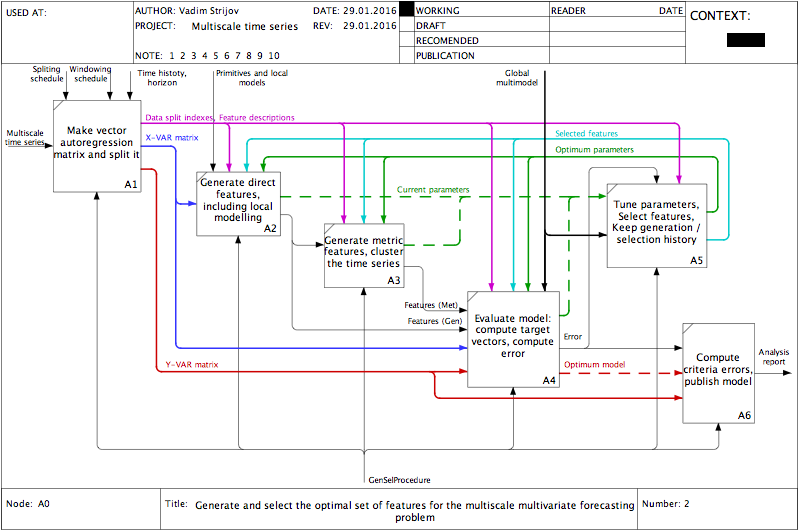
\includegraphics[width=0.9\textwidth]{02_A0.png}
\label{fg:IDEF}
\caption{Multiscale forecasting pipeline.}
\end{figure}

\section{Appendix: Discrete genetic algorithm for feature selection (will be converted to bootstrap random linear multimodel algorithm)}
\begin{enumerate}
\item There are set of binary vectors $\{\mathbf{a}_1,\ldots,\mathbf{a}_P\}$, $\mathbf{a}\in\{0,1\}^n$;
\item get two vectors $\mathbf{a}_p, \mathbf{a}_q$, $p,q\in\{1,\ldots,P\}$;
\item chose random number $\nu\in \{1,\ldots,n-1\}$;
\item split both vectors and change their parts:
$$[a_{p,1},\ldots,a_{p,\nu},a_{q,\nu+1},\ldots,a_{q,n}]\to\mathbf{a'}_p,$$
$$[a_{q,1},\ldots,a_{q,\nu},a_{p,\nu+1},\ldots,a_{p,n}]\to\mathbf{a'}_q;$$
\item choose random numbers $\eta_1,\ldots,\eta_Q\in\{1,\ldots,n\}$;
\item invert positions $\eta_1,\ldots,\eta_Q$ of the vectors $\mathbf{a'}_p,\mathbf{a'}_q$;
\item repeat items 2-6 $P/2$ times;
\item evaluate the obtained models.
\end{enumerate}
Repeat $R$~times; here $P,Q,R$ are the parameters of the algorithm and~$n$ is the number of the corresponding model features.

\section{Appendix: Mixture modelling under random bootstrapped models}
Denote the indexes of objects as $\{1,\ldots,i,\ldots,m\}=\I$, the split $\cI=\cB_1\sqcup\dots\sqcup\Bi_K$ and the indexes of  features as $\{1,\ldots,j,\ldots,n\}=\cJ$, the active set $\cA_k\subseteq\cJ$.

Let the regression model
\[
\fx:(\bw,\bx) \mapsto \by;
\]
with the selected model of optimal structure
\[
\quad \mathsf{E}(\by_i|\bx) = \bW_\cA\bx_i.
\]
The multimodel~$\mathfrak{f}$ is a set of the models~$\mathfrak{f}=\{\fx_k\quad | k=1,\ldots,K\}$, such that for each~$k$
\[
\mathsf{E}(y_{i\in\cB_k}|\bx) = \bW_{\cA_k}\bx_{i\in\cB_k}
\qquad\text{with}\quad \cI=\sqcup_{k=1}^K\cB_k\ni{i}.
\]
State the multimodel selection problem as follows. An optimal single model is
\[
\hat{\fx}(\bw,\bx) = \arg\max\limits_{\cA\subseteq\cJ}\mathcal{E}\left(\fx(\bw_\cA,\bx)\right),
\]
where~$\mathcal{E}$ denotes the model evidence in coherent Bayesian inference.
An optimal multilevel model i s
\[
\hat{\mathfrak{f}}(\bw_1,\ldots,\bw_K,\bx) = \arg\max\limits_{\sqcup_{k=1}^K\cB_k=\cI}\prod_{k=1}^K\mathcal{E}\left(\fx(\bw_k,\x_{\cB_k})\right).
\]

\sout{The model difference must be statistically significant}
\[
\mathcal{F}\supset\hat{\mathfrak{f}} = \arg\max\limits_{\cB_1,\cB_2\subset\cB}
\rho(f_1,f_2)
\]
\sout{given set of indices~$\hat{\Aj}$, such that}
\[
\hat{\cA} = \arg\max\limits_{\cA\subseteq\cJ}\mathcal{E}\left(\fx_1(\bw_\cA,\x^{\cB_1})\right)\mathcal{E}\left(\fx_2(\bw'_\cA,\bx^{\cB_2})\right).
\]



\end{document}

Constructing the object dictionary

According to the hypothesis ``the deeper history the lesser its impact to the future�� start forming the sample set~$X$ form the present time to the past expecting consequential augmentation of the forecasting quality.
\begin{def}
Call the necessary sample size the size when the augmentation of the forecasting quality probabilistically converges on the sample set increasing. Note that the sample set must be simple: there exist a single adequate model, which approximates the whole set.
\end{def}

\begin{def} Call the model stability the
\end{def}

\begin{def} Call the multimodel stability
\end{def}

Basic model
(Short description of the random forest)



\end{document} 